\documentclass{UoYCSproject}

\usepackage[backend=biber]{biblatex}
\usepackage{graphicx}
\usepackage{float}
\usepackage{booktabs}
\usepackage{caption}
\usepackage{listings}
\usepackage{color}
\usepackage{amsmath}
\usepackage{algorithm}
\usepackage[noend]{algpseudocode}

\newcommand{\ra}[1]{\renewcommand{\arraystretch}{#1}}
\renewcommand{\algorithmicrequire}{\textbf{Input:}}
\renewcommand{\algorithmicensure}{\textbf{Output:}}

\addbibresource{references.bib}
\author{Sophie Wood}
\title{Model-driven software migration between microcontrollers}
\date{Version 0.1, 2018-May-16}
\supervisor{Simos Gerasimou}
\SWE
% TODO update wordcount
\wordcount{0}

% TODO update includes/excludes
\includes{Appendices TODO}

\excludes{TODO}

% TODO update abstract
\abstract{TODO}

% TODO update acknowledgements
\acknowledgements{TODO}

%TODO add statement of ethics

\begin{document}
\maketitle
\listoffigures
\listoftables

\chapter{Introduction}
\section{Background and Motivation}

Bartels et al. define obsolescence as ``materials, parts, devices, software, services and processes that become non-procurable from their original manufacturer or supplier'' \parencite{bartels2012strategies}. Both software and hardware can be subject to obsolescence problems. 

Issues with hardware obsolescence have been driven by the growth of the electronics industry. This has reduced the life cycle of electronic parts as competitors release products with better functionality and features. Existing products are no longer commercially viable and therefore go out of production \parencite{bartels2012strategies}. This is a particular issue in the defence/aerospace sectors as the typical life cycle of a system is 20-30 years or longer \parencite{rojo2010obsolescence}. As such, parts will become unavailable before the system is completed. Singh et al. found that these systems ``often encounter obsolescence problems before they are fielded and always during their support life'' \parencite{singh2006obsolescence}.

Obsolescence is also a concern in the software industry. Businesses must continuously update their products in order to stay ahead. Bill Gates has said: 
\begin{quote}
``The only big companies that succeed will be those that obsolete their own products before someone else does.'' \parencite{bartels2012strategies}
\end{quote}
There are three main causes of software obsolescence: \textit{logistical} -  digital media obsolescence, formatting or degradation terminates or limits access to software; \textit{functional} - hardware, requirements, or other software changes to the system obsolete the functionality of the software; and \textit{technological} - the sales and/or support for commercial off the shelf (COTS) software terminates \parencite{sandborn2007obsolescence}. 

In addition, software obsolescence can be driven by hardware obsolescence and vice versa. Another issue is lack of skills. For example, there may be a limited number of people that are competent in the language the system is written in. If these people leave the company, the system can no longer be maintained \parencite{rajagopal2014software}. 

Again avionics/military and other ``safety-critical'' systems particularly struggle with software obsolescence issues as even small changes may have to go through extensive and costly qualification/certification processes \parencite{singh2006obsolescence}. Consequently, software obsolescence costs can equal or exceed that of hardware \parencite{sandborn2007obsolescence}. Despite this, strategies for obsolescence mitigation/management have generally focused on hardware obsolescence problems. It is important that both hardware and software obsolescence issues are tackled as these problems can be incredibly costly to these industries. For example, the US Navy estimates that obsolescence problems can cost up to \$750 million annually \parencite{adams2005getting}. Sandborn and Myers also found that sustainment costs (which include costs related to obsolescence) dominate the system costs in the case of development of an F-16 military aircraft \parencite{sandborn2008designing}. 
 
Current strategies for mitigating software obsolescence issues are insufficient. Proactive measures (e.g. improving code portability or using open-source software) often require either a large amount of resources or resources that are unavailable. Reactive strategies for tackling obsolescence (e.g. software license downgrades, source code purchase or third party support) may not always be possible. When these methods are inadequate, the legacy system may have to be redeveloped or rehosted \parencite{sandborn2007obsolescence}. However, many such software modernisation projects are abandoned or not completed within the planned timescale/budget \parencite{kowalczyk2009model}. 

If redevelopment projects can be automated or even partially automated, they can more easily be completed on time. \parencite{gerasimou2017technical} uses code analysis and code-based transformations to partially automate the process of adapting software to work with different libraries as well as migrating software between hardware platforms. Although this approach is successful, the process may not scale well. For example, in one stage of the process of adapting code to use a new library, an abstraction layer is generated that has the same usage behaviour as the obsolete library. This is then used to replace the usages of the legacy library. If applied to a project with many library usages, this could generate a large amount of additional code in the modernised project which may make it difficult to maintain. 

An alternative approach is to use model-driven software modernisation (MDSM) for (partial) automation of modernisation projects. MDSM is based on the use of model-driven engineering (MDE) principles such as models and transformations to facilitate the migration process (MDE and its application to software modernisation are discussed in more detail in Sections \ref{mde_approaches} and \ref{mde_bg}). For example, model-to-model transformations can be used to map a model of the legacy code to a model of the new system. A model-to-text transformation can then be applied to this new model to generate code for the new version of the system.

MDSM is a promising approach as it has already been proved feasible in industry by the Sodifrance\footnote{https://www.sodifrance.fr/} company. For example, they were able to migrate a large-scale banking system (at a size of around one million lines of code) to J2EE \parencite{fleurey2007model}. Kowalczyk and Kwieci\'nska have also demonstrated the viability of MDSM by modernising a project written in Java 1.4 and the Hibernate 2.x framework into Java 1.5 and Hibernate 3.x \parencite{kowalczyk2009model}. One benefit of MDSM is that tools (e.g. model discoverers) can sometimes be reused between projects making subsequent modernisation projects quicker and cheaper to complete. For example, MoDisco is an open-source model-discoverer that can generate models from Java code \parencite{bruneliere2014modisco}.

The Defence Science and Technology Laboratory (DSTL) at the Ministry of Defence (MoD) have identified several instances of software obsolescence they would like to tackle. A problem of particular interest is ``the migration of an entire software system from a legacy hardware platform to a modern more powerful platform'' \parencite{gerasimou2017technical}. This report will explore how MDSM processes can be used to partially automate the migration of code between microprocessors. A case study implementing the migration of code between a Parallax Propeller Activity Board and an Arduino Uno will be used to demonstrate the approach developed.
 
\section{Project Goals}
TODO
\section{Project Scope}
TODO
\section{Report Structure}
TODO

\chapter{Literature Review}
The following chapter introduces the existing work on software obsolescence and the technical background required to understand this project. It begins with an overview of the existing approaches for software obsolescence mitigation in Section \ref{so_approaches} and in particular, MDE-based strategies in Section \ref{mde_approaches}. The specific problem of migration between microcontrollers and the existing methods for facilitating this are discussed in Section \ref{mc_migration} as well as how the MDSM-based method explored in this project is related. 

Sections \ref{mde_bg} and \ref{mc_bg} contain the technical background of the project including a brief overview of MDE and the chosen framework for this project as well as a description of the microcontrollers used for the case study.

\section{Existing Work}
\subsection{Approaches to Software Obsolescence} \label{so_approaches}
Rojo et al. identify some of the main methods of tackling obsolescence in their paper ``Obsolescence management for long-life contracts: state of the art and future trends'' \parencite{rojo2010obsolescence}. Although they identified many strategies for handling the obsolescence of electronic components, very few methods were relevant for dealing with software obsolescence.

The tools ``se-Fly Fisher'' and ``R2T2'' (Rapid Response Technology Trade) were identified as useful for managing software obsolescence. These tools are used for design refresh planning. Design refresh planning deals with obsolescence in a proactive manner by planning the best times for performing a redesign of the system during the sustainment stage of its lifecycle. 

Se-Fly Fisher uses the technology curves of each part of the system to: forecast how often a system baseline should change; identify replacement resources and estimate the benefit of each system baseline change \parencite{rojo2010obsolescence}.

Similarly, R2T2 can: forecast system obsolescence; allow for comparisons to alternative solutions; produce a life cycle obsolescence plan for the elements that require refreshment and plan when element replacements should occur \parencite{herald2009obsolescence}.

These forecasting tools may enable organisations to plan ahead and handle cases where equivalent parts/software are available. However, they cannot assist in the actual redesign or redevelopment process which can be time consuming and costly.

Similarly, Sandborn et al. identified very few approaches towards managing software obsolescence. The main methods they identified for mitigating software obsolescence were \parencite{sandborn2007obsolescence}:
\begin{description}
\item[(1) Software License Downgrade:] users can purchase licenses for the current product and apply them to older versions.
\item[(2) Source Code Purchase:] customers purchase the source code for the product.
\item[(3) Third Party Support:] a third party is contracted to maintain support for the software.
\end{description}
When possible, these approaches could reduce costs as the software does not have to be maintained in house or redeveloped. However, sometimes these methods may not be possible. Additionally, given that the system owners are so dependent on the legacy code, it puts them in a poor position for negotiating the prices for these contracts and so this approach could become costly.

\subsection{MDE Approaches to Software Obsolescence} \label{mde_approaches}
More recently, MDE approaches have been used to tackle software obsolescence problems where legacy code must be redeveloped. MDE allows some of the stages in migration to be automated, consequently reducing the timescale and costs involved.

The company Sodifrance has successfully been using MDE for development and migration projects for over ten years \parencite{fleurey2007model}. The general MDE approach to migration used by Sodifrance is shown in Figure \ref{fig:sodifrance_process}. The approach is separated into four stages as follow:

\begin{enumerate}
\item Firstly, the code of the legacy application is parsed in order to create a model of the legacy system. In Figure \ref{fig:sodifrance_process}, \textit{L} indicates the metamodel for the implementation language of the legacy code.
\item This model is then transformed to a Platform Independent Model (PIM) conforming to an ANT metamodel\footnote{An ANT metamodel contains packages to represent:
\begin{itemize}
\item Static data structures (close to the UML class diagram).
\item Actions and algorithms (it includes an imperative action language).
\item Graphical user interfaces and widgets.
\item Application navigation.
\end{itemize}}. This model represents a high-level view of the legacy code. This process is dependent on knowledge of the libraries and coding conventions used by the legacy platform.
\item Next the PIM has a model transformation applied to produce a Platform Specific Model (PSM) conforming to a UML metamodel. The high-level views from the PIM are adapted to fit the target platform.
\item Finally, code is generated from the PSM by using template-based text generation tools.
\end{enumerate}

\begin{figure}[h!]
  \centering
  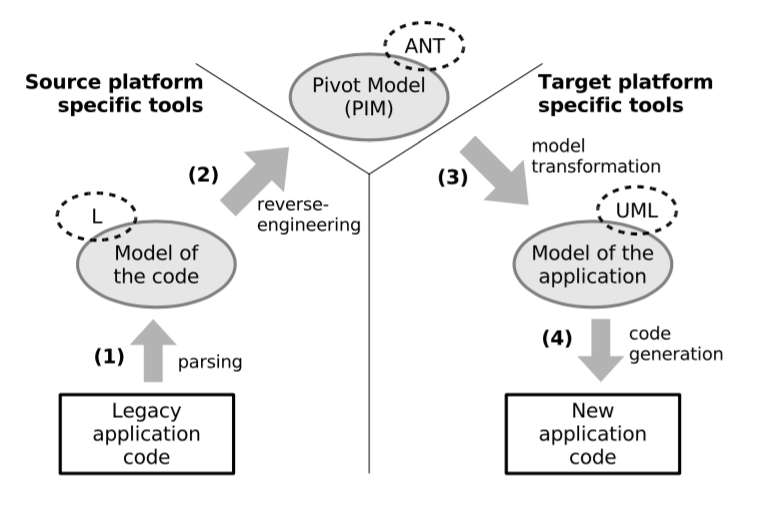
\includegraphics[width=0.6\linewidth]{graphics/sodifrance_mde.png}
  \caption{The general model-driven migration process used by Sodifrance \parencite{fleurey2007model}.}
  \label{fig:sodifrance_process}
\end{figure}

The first two steps of the process can usually be fully automated. However, the remaining stages need some manual effort. Tasks that could not be completed automatically are indicated in the generated code (e.g. by TODO directives in Java applications) and summarised into a task list in order to allow the manual process to be completed more efficiently.

Sodifrance demonstrated the effectiveness of their approach using a case study of migrating a large-scale banking system from Mainframe to J2EE.

Kowalczyk and Kwieci\'nska have also explored the use of MDE in software migration \parencite{kowalczyk2009model}. They identified two main approaches: the ``Reverse MDA approach'' (RMA) and the ``Direct Transformation Approach'' (DTA).

The RMA approach follows the same stages as that used by Sodifrance. The DTA approach shown in Figure \ref{fig:dta} reduces the number of stages involved in the transformation process by directly transforming between platform specific models. 

\begin{figure}[h!]
  \centering
  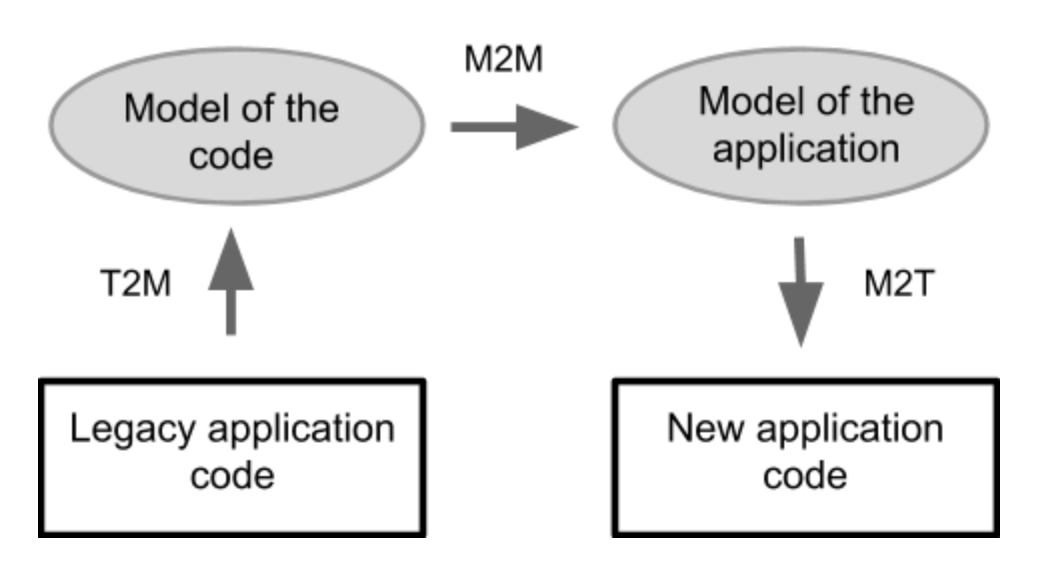
\includegraphics[width=0.6\linewidth]{graphics/dta.png}
  \caption{The stages involved in the ``Direct Transformation Approach''.}
  \label{fig:dta}
\end{figure}

The feasibility of both approaches was demonstrated by a case study migrating from Java 1.4 and the Hibernate 2.x framework to Java 1.5 and Hibernate 3.x. Based on qualitative analysis of the two approaches, they recommend to use an approach similar to DTA as it is often not the case that a transformation from the legacy code model to the PIM will exist. It is especially suited to cases where the code model and application model use the same metamodel. 

MDE approaches to software migration have many benefits. The primary reason is the ability to automate some of the stages in the migration process, consequently reducing the cost and time scale of projects. Secondly, parts of the process (e.g. model discoverers or transformations) can be reused between different migration projects which will again cut the cost of migration.

There are however, drawbacks to the MDE approach. There is a high cost of entry to start using MDE methods --- the initial development of processes and tools can be time consuming and expensive if open-source tools are not available. Secondly, a particular issue in commercial projects is that no code will be available until the initial analysis and tool development stage of the process is completed. In the case of the Sodifrance case study, code was not delivered until 10 months after the project had begun \parencite{fleurey2007model}. This can make customers nervous and reluctant to try this approach. On the other hand, once the initial stage is completed, the delivery rate of the code can be much faster than for a standard re-development approach.

One of the main considerations that must be made when choosing an MDE approach is the size of the project. If the project is small, it may be more expensive to use this method as the initial stages may take longer than manually migrating the code \parencite{fleurey2007model}. This is demonstrated in Figure \ref{fig:costvsize}.

\begin{figure}[h!]
  \centering
  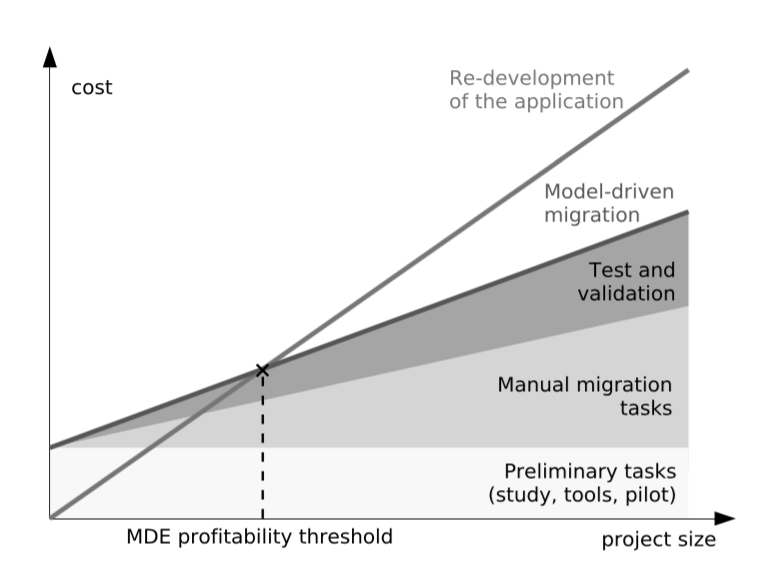
\includegraphics[width=0.6\linewidth]{graphics/costvsize.png}
  \caption{Project migration cost as a function of its size \parencite{fleurey2007model}.}
  \label{fig:costvsize}
\end{figure}

\subsection{Migration Between Microcontrollers} \label{mc_migration}
As mentioned previously, a particular problem of interest to the MoD is ``the migration of an entire software system from a legacy hardware platform to a modern more powerful platform'' \parencite{gerasimou2017technical}.

Atmel addressed the issue of migrating code between microcontrollers by reducing the learning curve for developers moving from development on 8-bit to 32-bit platforms. They aimed to achieve this by providing powerful debug facilities and development tools similar to established 8-bit development platforms \parencite{wilbrink2004facilitating}.

Although this strategy should reduce the migration effort, the code will still be have to be migrated manually which is error-prone and difficult. Additionally, the development of new tools adds extra overhead to the project, although these tools are reusable between projects.

Another approach for migrating code between microprocessors combines code analysis, code-based transformations and verification/validation techniques \parencite{gerasimou2017technical}. The procedure follows the following steps:
\begin{description}
\item[(1) Software system analysis (automated):] The source code and obsolete libraries are parsed to obtain abstract syntax trees (ASTs). The AST can be examined to indicate the elements using the obsolete library and help establish the system's dependency level.
\item[(2) Discovery of similar libraries (non-automated):] The development team identifies candidate libraries for replacement of the obsolete library.
\item[(3) Compatibility analysis of the discovered libraries (non-automated):] Candidate libraries are rejected if they don't conform to technical or semantic requirements.
\item[(4) Data visualisation (automated):] Used to analyse the software system and its coupling with the obsolete library.
\item[(5) Execute generation transformations (automated):] Firstly, an abstraction layer is generated that has the same usage behaviour as the obsolete library. Next the obsolete library usages are replaced with this abstract layer.
\item[(6) Mappings inference (non-automated):] A developer creates a list of mapping rules by inspection of the obsolete and replacement libraries.
\item[(7) Code population (non-automated):] A developer uses the mapping rules generated in stage 6 to populate the abstraction layer generated in stage 5.
\end{description}
This method was demonstrated to succeed in partially automating the migration of software between an Arduino and Raspberry Pi.

By automating some of the migration stages, the overall time and cost of software modernisation should be reduced. Another benefit is that the code analysis stages allow for potential risks to be detected early on. However, there is still a lot of manual effort required for migrating between libraries and in particular, generating mapping rules requires a developer with a strong understanding of both the new and obsolete libraries. Another issue is that adding the abstraction layer could lead to a large increase in the size of the code if the obsolete libraries are used frequently. This could make the code more difficult to maintain.

My project aims to explore an alternative approach for migrating code between microcontrollers by applying an MDE approach similar to that discussed in Section \ref{mde_approaches}. In doing so I aim to be able to (partially) automate the migration process, consequently reducing the time taken for migration whilst also avoiding issues associated with other methods such as code blow-up in \parencite{gerasimou2017technical}.

\section{Model Driven Engineering} \label{mde_bg}
Model Driven Engineering (MDE) was developed in order to address complexity within the problem space of computing. In the past, approaches for enabling programmers to develop code more easily have focused on simplifying the solution space. This was achieved by providing abstractions such as higher-level programming languages or providing operating systems to manage the difficulty of programming hardware directly. However, these solutions are unable to express domain concepts effectively, unlike MDE techniques \parencite{schmidt2006model}. Furthermore, it has been found that MDE can also be utilised in automating the software development process \parencite{bezivin2004search}.
\newline
The rest of this section introduces the terminology and main components of MDE as well as the MDE framework I will use in the project.

\subsection{Domain-Specific Modelling Languages (DSMLs)}
Meta-meta-modelling mechanisms such as the Object Management Group's (OMG) Meta Object Facility (MOF) can be used to create modelling languages for a given problem domain \parencite{mussbacher2014relevance}. The key components of the OMG's approach to DSMLs are \parencite{bezivin2001towards}:
\begin{description}
\item[Models:] A model is a simplification of a system built with an intended goal in mind. Models should be easier to use than the original system. This is achieved by abstracting out details of the system that are unnecessary for the target model's intended purpose.
\item[Meta-models:] A meta-model is the explicit specification of an abstraction (i.e. model). 
\item[Meta-meta-models:]  A meta-meta-model is used to define meta-models. In particular, the OMG define the MOF (Meta Object Facility) which is a self-defined meta-meta-model.
\end{description}

The relationships between these MDE concepts are summarised in Figure \ref{fig:metamodel_term}

\begin{figure}[h!]
  \centering
  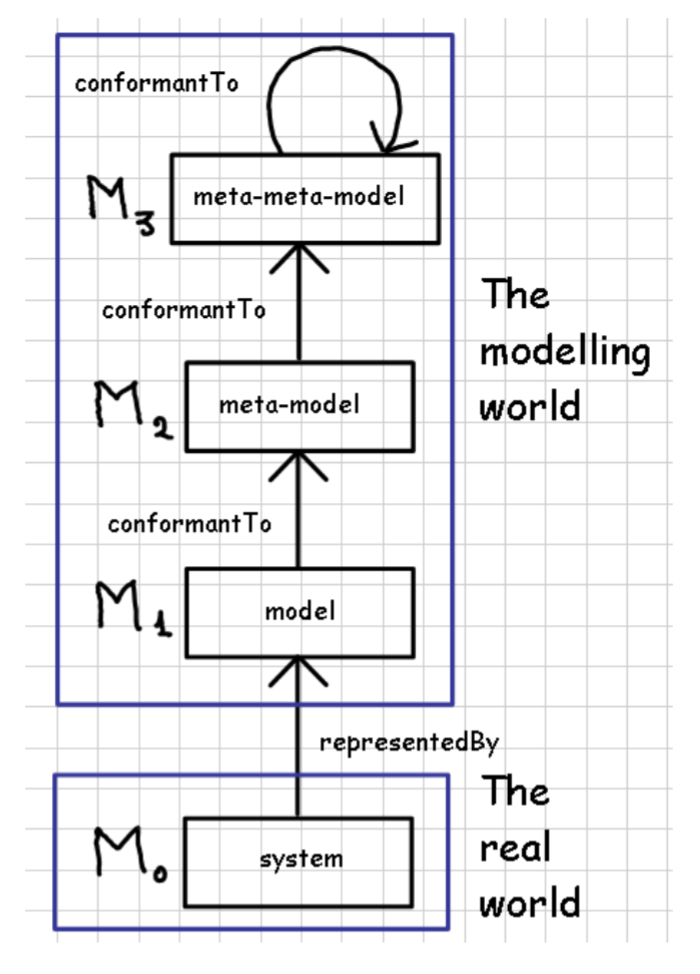
\includegraphics[width=0.5\linewidth]{graphics/metamodel_terminology.png}
  \caption{The relationship between the key concepts in MDE \parencite{bezivin2004search}.}
  \label{fig:metamodel_term}
\end{figure}


\subsection{Model Transformations}
There are three main categories of model transformation:
\begin{description}
\item[Model-to-model (M2M):] M2M transformations are used to translate source models to target models. The source and target models can be instances of the same or different meta-models \parencite{czarnecki2003classification}.
\item[Model-to-Text (M2T):] These can be considered a special case of M2M transformations. It is often the case that M2T transformations are used for code generation. The most common approach to M2T transformation is a template-based approach. A template contains mixtures of static text and dynamic sections that can be used to access information from the source model \parencite{czarnecki2003classification}.
\item[Text-to-Model (T2M):]  T2M transformations can be used to transform code to a model (conforming to a language meta-model). Model discoverer tools such as MoDisco \parencite{bruneliere2014modisco} are the easiest way to perform T2M transformations on code \parencite{kowalczyk2009model}.
\end{description}

\subsection{The Epsilon Framework}
% TODO may be worth comparing to M2T Xpand
Epsilon is a family of programming languages for model management tasks. It provides (among others) the following languages of interest \parencite{kolovos2010epsilon}:
\begin{description}
\item[Epsilon Object Language (EOL):] EOL is the common basis for the languages provided by Epsilon. It can be used for querying and modifying models.
\item[Epsilon Validation Language (EVL):] EVL is used for model validation.
\item[Epsilon Transformation Language (ETL):] ETL is used for M2M transformations.
\item[Epsilon Generation Language (EGL):] EGL is used for M2T transformations.
\end{description}
Epsilon also enables the use of ANT tasks to create workflows of different tasks (e.g. a validation followed by a
transformation followed by code generation) \parencite{kolovos2010epsilon}.
\newline
Epsilon has been chosen as the framework for this project over others for the following reasons:
\begin{itemize}
\item It is well documented with many tutorials as well as ``The Epsilon Book'' being freely available. Additionally, there is an active forum for any questions not answered by these sources \parencite{epsilonsite}.
\item It is well integrated with Eclipse (for example, syntax/error highlighting is provided in the editor and there are graphical tools for running/debugging programs) and has been an official project since 2006 \parencite{epsilonsite}.
\item Epsilon provides a connectivity layer (EMC). This layer allows EOL programs to access models of different modelling technologies including Eclipse Modelling Framework (EMF) models and XML documents \parencite{epsilonsite}.
\item I am already familiar with how to use the framework.
\end{itemize}

\section{Microcontroller Background} \label{mc_bg}
The project involves migration of code from a Parallax Propeller Activity Board to an Arduino Uno. However, since some features of the boards are different, this must be taken into account when migrating code. For example, the Propeller Activity Board has 16 digital pins whereas the Arduino Uno only has 14. In this case, code may need to be adapted to use different pins on the Arduino if it is migrated from the Propeller Activity Board. The following section highlights the important features and differences between the two boards as well as an overview of the board layout.

\subsection{Parallax Propeller Activity Board}
\begin{figure}[h!]
  \centering
  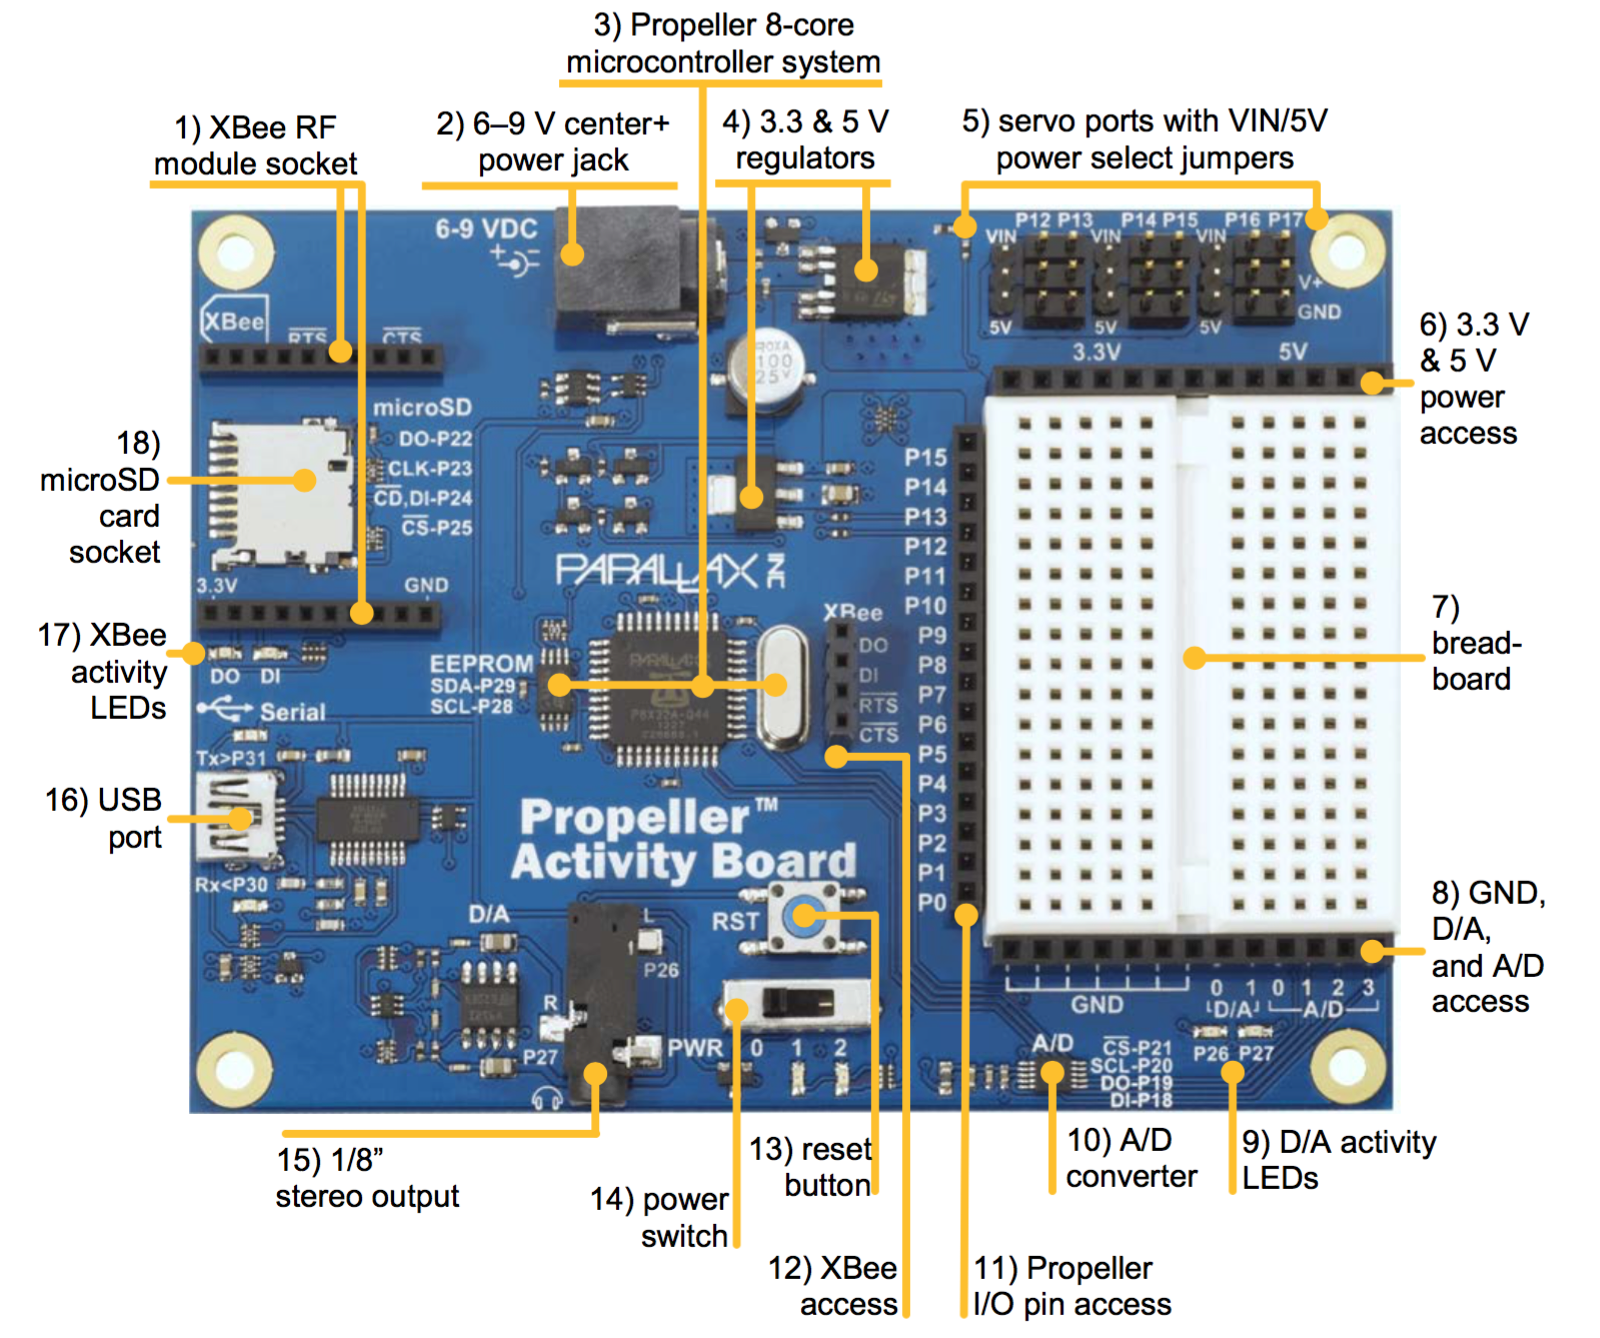
\includegraphics[width=0.6\linewidth]{graphics/propeller_board.png}
  \caption{Features of the Parallax Propeller Activity Board \parencite{propellerspec}.}
  \label{fig:prop_board}
\end{figure}

The key features of the Parallax Propeller Activity Board are \parencite{propellerspec}:
\begin{itemize}
\item Built-in 8-core Propeller P8X32A microcontroller
\item 64KB EEPROM
\item XBee wireless module socket
\item 16 digital I/O pins
\item 4 Analog-to-Digital pins
\item 2 Digital-to-Analog pins
\end{itemize}

\subsection{Arduino Uno}
%TODO: figure out which version I will be using
\begin{figure}[h!]
  \centering
  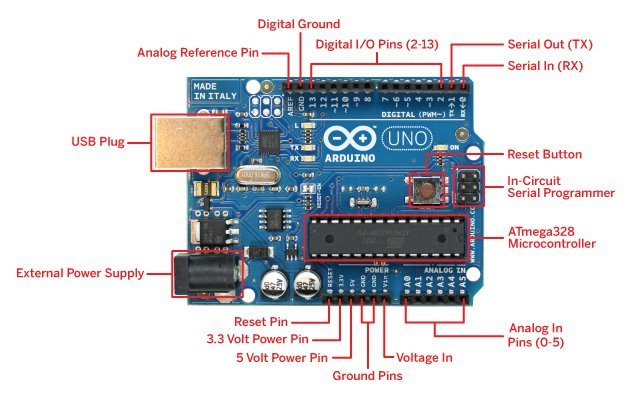
\includegraphics[width=0.8\linewidth]{graphics/arduino_board.jpg}
  \caption{Features of the Arduino Uno \parencite{arduinodiagram}.}
  \label{fig:arduino_uno}
\end{figure}

The key features of the Arduino Uno are \parencite{arduinospec}:
\begin{itemize}
\item Built-in single-core ATmega328 microcontroller
\item 32KB flash memory
\item 2KB SRAM
\item 1KB EEPROM
\item 14 digital I/O pins (6 provide PWM output)
\item 6 analog input pins
\end{itemize}

\chapter{Methodology}
This section summarises the methodology and tools used for managing this project. It begins with an overview of project management methodologies in Section \ref{overview_meth} and discusses the methodology chosen for this particular project in Section \ref{choice_meth}. Finally, the tools used for project management are discussed in Section \ref{proj_mgmt}.

\section{Overview of Methodologies} \label{overview_meth}
Project management methodologies can be roughly categorised as either traditional or agile methodologies. Each have their own strengths and weaknesses. Sections \ref{trad_meth} and \ref{agile_meth} provide an overview of these methodologies.
\subsection{Traditional Methodologies} \label{trad_meth}
Traditional approaches include the waterfall/linear methodology and the incremental strategy. The common features of these methodologies are that they are very structured and there is little room for deviation from the original plan. For example, the waterfall methodology splits the project into separate stages for software requirements gathering, systems requirements gathering, analysis, design, coding, testing and operations such that each section is completed before the next begins \parencite{royce1987managing}.

These strategies are best suited to projects that have a clear goal and clear solution. In this case, the use of these strategies can have many benefits. For example, the entire project is scheduled and resource requirements are known from the beginning. Additionally, this allows for team members to be distributed \parencite{fernandez2008agile}. However, heavy documentation is required and a detailed plan is needed from the start of the project. As such, it is difficult to adapt this pan to changes in requirements \parencite{fernandez2008agile}.

\subsection{Agile Methodologies} \label{agile_meth}
Agile methodologies are generally better at accommodating change than traditional methodologies as they repeatedly return to earlier stages in the development process. For example, Figure \ref{fig:agile_meths} shows a (simplified) view of the stages involved in the iterative, adaptive and extreme agile methodologies. Each approach goes through the full development process, tests and/or deploys the system (or a part of the system) and optionally returns to either the build, design or scope stage depending on the outcome of testing and deployment. This cycle can occur multiple times in the project lifecycle and is referred to as a sprint. Sprints generally last a few weeks but this can vary depending on the project.

\begin{figure}[h!]
  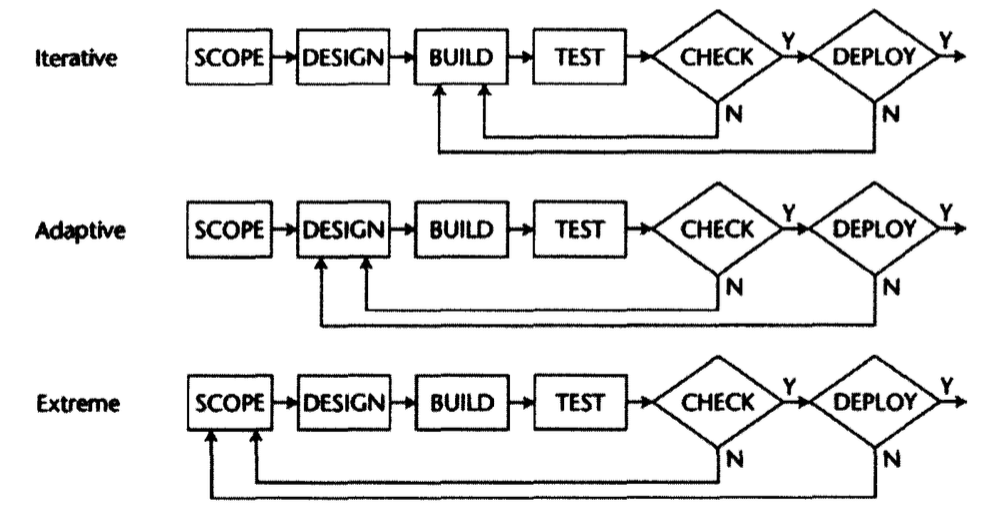
\includegraphics[width=\linewidth]{graphics/agile_methodologies.png}
  \caption{An overview of the iterative, adaptive and extreme agile methodologies \parencite{fernandez2008agile}.}
  \label{fig:agile_meths}
\end{figure}

As previously mentioned, the ability to return to earlier stages in the development process can help accommodate changing requirements. For example, the client can review what is produced at the end of each sprint and clarify or change requirements depending on the outcome. However, an agile approach requires much closer communication with the client which may not always be possible or desirable. Additionally, since requirements are not fixed for the duration of the project, the final product is not always clear from the start of the project \parencite{fernandez2008agile}.

\section{Choice of Methodology} \label{choice_meth}
The approach for this project is fairly well defined i.e. an MDE-based method will be used to perform software migration. However, the requirements are likely to change throughout the course of the project depending on the success of system prototypes. As such, the project is more suited to an agile methodology as this can more easily manage these changes. Additionally, I will be meeting with the project supervisor weekly which will allow us to work on updating the requirements as necessary and allows the project to be easily split into sprints beginning and ending at these meetings. In particular, the extreme methodology will be the most suitable as it allows for changing the scope which may be required if early research indicates the scope is unsuitable for the time allocated.

\section{Project Management} \label{proj_mgmt}
This section discusses the tools used in order to manage the project. This includes tools for task management as well as version control tools for the source code and report.

At the start of the project a GANTT chart was created in order to give a rough estimate for when certain parts of the project would be completed. This was not updated throughout the project and doesn't particularly fit with the agile methodology but it was helpful to ensure progress was being made at about the right pace. In particular, this was helpful for writing the report.

The GANTT chart was included in the project page which was created using Google Sites. This page was used to contain all the information for managing the project. In particular it was used for organising the literature review but also links to the task management tool for the project. Google Sites was chosen as it is free and can be easily adapted to suit the project. The literature review was organised by creating pages on the site for each category within the literature review (e.g. MDE background) and collecting notes from the relevant papers on these pages. The site also contained a list of papers to be read and a link to the Trello board for managing the writing and coding tasks. Trello is used as it is free and makes it easy to prioritise and organise tasks.

Git was used as the version control system for both the source code of the system and the documentation as it is free and I already had experience using it. The remote repositories were hosted on GitHub as it allows students to use private repositories for free. In particular, Git was chosen for managing the documentation over e.g. Google Drive as the report was written in \LaTeX~and so updates to the main report document could require changes to e.g. image files or the bibliography file. As such, it is easier to backup all these files at once using a single Git command rather than adding and deleting files from Google Drive. Additionally, the file history is saved using Git so it is easier to return to previous versions of the documentation.

\chapter{Requirements} \label{reqs}
This chapter discusses the requirements that must be satisfied in order to consider the project successful. Firstly, Section \ref{req_gathering} introduces the sources used to derive requirements including the relevant stakeholders for the project. Then Sections \ref{stakeholder_reqs} and \ref{sys_reqs} summarise the stakeholder and system requirements respectively. Each requirement is assigned an identifier and a priority based on the MoSCoW categorisation system \parencite{moscow}. In decreasing order, the priority levels each requirement can have are \textbf{M} (must have), \textbf{S} (should have), \textbf{C} (could have) and \textbf{W} (won't have).

\section{Requirements Elicitation} \label{req_gathering}
This section discusses the main sources considered for deriving requirements. Firstly, a summary of the initial project statement is presented in Section \ref{proj_stmt} as this is helpful for deriving the functional requirements for the project. Secondly, stakeholders for the project are identified in Section \ref{stakeholders} in order to enable gathering of stakeholder requirements.

\subsection{Project Statement} \label{proj_stmt}
The initial project statement is as follows: 
\begin{quote}
``This project aims to design and develop an extensible MDE-based infrastructure for migrating software applications between microprocessors. In particular, the project will enable:
\begin{itemize}
\item analysis and extraction of source code deployed on the old microprocessor
\item migration of extracted source code to the new microprocessor''
\end{itemize}
\end{quote}

\subsection{Stakeholders} \label{stakeholders}
Stakeholders are parties that are interested in the development of the project and therefore their goals must be taken into account when deriving requirements. The rest of this section introduces the roles of the primary stakeholders and gives a high-level overview of their objectives for the project.

\begin{description}
\item[Student/Project Developer:] Responsible for research, system design, development and testing. Primarily interested in demonstrating the efficacy of an MDE based approach to software migration and successfully completing the project on time.

\item[Project Supervisor:] Responsible for meeting regularly with the student and guiding the research for the project. Their goal is also for the system to be finished within schedule.

\item[Software Obsolescence Researchers:] Although not directly involved in the project, the results of the project may be of interest to researchers in the field of software obsolescence. In particular, the project explores an alternative approach to the migration of software between microcontrollers presented in \parencite{gerasimou2017technical}. This is a particular problem of interest to the DSTL. However, they are specifically investigating migration between their own microcontrollers such as the FS P4080. Therefore, they would require that the system is easily understandable and can be adapted to work with microcontrollers other than the Parallax Propeller Activity Board and the Arduino Uno.

\item[End Users:] No end users are directly involved in the project. However, some people may want to use the resulting system as is to migrate software from a Parallax Propeller Activity Board to an Arduino Uno. In this case, their main priority would be usability of the system. Additionally, it is important that the performance of the migrated software is not significantly worse than the source application. However, as this is a very specific scenario, it is unlikely that this user group will be very large. Similarly to software obsolescence researchers, it may be more useful to end users if the system can be easily modified to support migration between microcontrollers other than the Parallax Propeller Activity Board and Arduino Uno.
\end{description}

\section{Stakeholder Requirements} \label{stakeholder_reqs}
Table \ref{table:stakeholder_req} summarises the stakeholder requirements for the system. Each requirement has an identifier of the form S-X (where X is an integer).
\begin{table*}[h!]\centering
\ra{1.3}
  \begin{tabular}{@{}p{0.1\textwidth}p{0.15\textwidth}p{0.75\textwidth}@{}} \toprule 
  \textbf{ID} & \textbf{Priority} & \textbf{Description} \\
  \midrule
  S-1 & M & Users can provide the system with the source code for a Parallax Propeller Activity Board and target code for the Arduino Uno will be generated. \\ 
  S-2 & M & Users can easily adapt the system to support migration of software between different microprocessors. \\
  S-3 & S & Users can easily determine sources of errors when using the system. \\
  S-4 & S & Users can easily identify areas of the target code that cannot automatically be migrated and must be manually completed. \\
  S-5 & S & The performance of the migrated code is not significantly worse than the source application. \\
  \bottomrule
  \end{tabular}
\caption{Stakeholder Requirements}
\label{table:stakeholder_req}
\end{table*}

\section{System Requirements} \label{sys_reqs}
The following section summarises the functional and non-functional requirements of the system. Each functional requirement is assigned an identifier of the form F-X (where X is an integer) and each non-functional requirement is assigned an identifier of the form NF-X (where X is an integer).

Note that valid source code refers to an application which compiles and runs correctly on the source microprocessor and only uses hardware capabilities provided by both microcontrollers.
\newpage
\subsection{Functional Requirements}
Table \ref{table:func_req} summarises the functional requirements and their acceptance criteria for the system.
\begin{table*}[h!]\centering
\ra{1.3}
  \begin{tabular}{@{}p{0.05\textwidth}p{0.1\textwidth}p{0.425\textwidth}p{0.425\textwidth}@{}} \toprule 
  \textbf{ID} & \textbf{Priority} & \textbf{Description} & \textbf{Acceptance Criteria} \\
  \midrule
  F-1 & M & The target microcontoller running the migrated code (potentially with manual additions) displays the same behaviour as the source microcontroller, provided the source code is valid. & Manual inspection of the migrated application confirms the behaviour is the same as the source application. \\
  F-2 & M & The migrated code deploys without errors on the target microcontroller if the provided source code is valid. & Manual inspection of the migration process confirms a valid source application can be migrated without errors. \\
  F-3 & S & The system displays appropriate errors when the source code cannot be migrated (e.g. there are errors in the source code or hardware incompatibilities). & Errors are thrown when invalid source code is provided to the migration process. \\  
  F-4 & S & The system clearly indicates any errors that have occurred during its use (e.g. the migration process fails). & Errors are thrown if the migration process fails. The errors clearly indicate the source of the problem. \\
  F-5 & S & The system should indicate any parts of the code that must be manually completed. & Manual inspection of the migrated code confirms that all parts of the code that must be manually completed are clearly indicated (e.g. by TODO directives). \\
  \bottomrule
  \end{tabular}
\caption{Functional Requirements}
\label{table:func_req}
\end{table*}

\subsection{Non-Functional Requirements}
Table \ref{table:non_func_req} summarises the non-functional requirements and their acceptance criteria for the system.
\begin{table*}[h!]\centering
\ra{1.3}
  \begin{tabular}{@{}p{0.08\textwidth}p{0.1\textwidth}p{0.41\textwidth}p{0.41\textwidth}@{}} \toprule 
  \textbf{ID} & \textbf{Priority} & \textbf{Description} & \textbf{Acceptance Criteria} \\
  \midrule
  NF-1 & M & The system should be easy to adapt to support migration between different microcontrollers. & Manual inspection of the system should indicate that it is easy to adapt. For example, if the system is based on an established MDE framework it will be easier to adapt as there will be more documentation available. \\
  NF-2 & S & The system should display a high-level of encapsulation. & Manual inspection of the system should indicate measures have been taken to facilitate encapsulation. For example, separation of hardware-dependent parts of the code. \\
  NF-3 & S & The migrated code should not be significantly larger than the source code. & Migrated code is of a size acceptable to the stakeholder. \\
  NF-4 & S & The migrated code should exhibit similar performance to the source code. & Migrated code runs in a duration acceptable for the stakeholder. \\
  
  \bottomrule
  \end{tabular}
\caption{Non-Functional Requirements}
\label{table:non_func_req}
\end{table*}

\newpage
\section{Requirements Traceability Matrix}
The requirements traceability matrix shown in Table \ref{table:traceability} shows how stakeholder requirements correspond to system requirements.
\begin{table*}[h!]\centering
\ra{1.3}
  \begin{tabular}{@{}p{0.4\textwidth}p{0.4\textwidth}@{}} \toprule 
  \textbf{Stakeholder Requirements} & \textbf{System Requirements} \\
  \midrule
  S-1 & F-1, F-2 \\
  S-2 & NF-1, NF-2, NF-3 \\
  S-3 & F-2, F-3, F-4 \\
  S-4 & F-5 \\
  S-5 & NF-4 \\
  \bottomrule
  \end{tabular}
\caption{Requirements Traceability Matrix}
\label{table:traceability}
\end{table*}

\chapter{Design and Implementation}
This chapter of the report discusses the decisions made in designing and implementing the system for supporting the migration of software from a Parallax Propeller Activity Board to an Arduino (these will be referred to as the source and target respectively). The system is implemented as an Eclipse plugin to assist in usability. Firstly, the high-level architecture of the plugin will be presented in Section \ref{high_lev_arch} along with the design rationale. This will be followed by an examination of the low-level architecture and implementation of these components in Sections \ref{fritz_design} to \ref{parallax_design}.


\section{High-Level Architecture} \label{high_lev_arch}
\begin{figure}[h!]
  \centering
  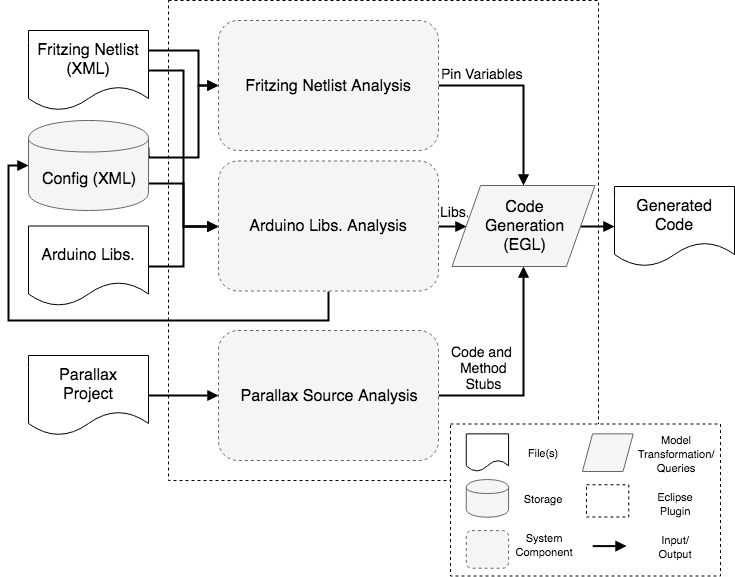
\includegraphics[width=0.8\linewidth]{graphics/high_level_overview.png}
  \caption{A high-level overview of the system.}
  \label{fig:high_level_overview}
\end{figure}

\subsection{Overview}
Figure \ref{fig:high_level_overview} shows the high-level architecture of the system. There are three main components to the system: Fritzing netlist analysis, Arduino libraries analysis and Parallax source code analysis. Each of these components produces information that contributes to code generation. The code generation is coordinated by an EGL transformation that takes the data from these components and generates a C file as output. This file acts as a basis for code that is compatible with the target platform. 

\begin{figure}[h!]
  \centering
  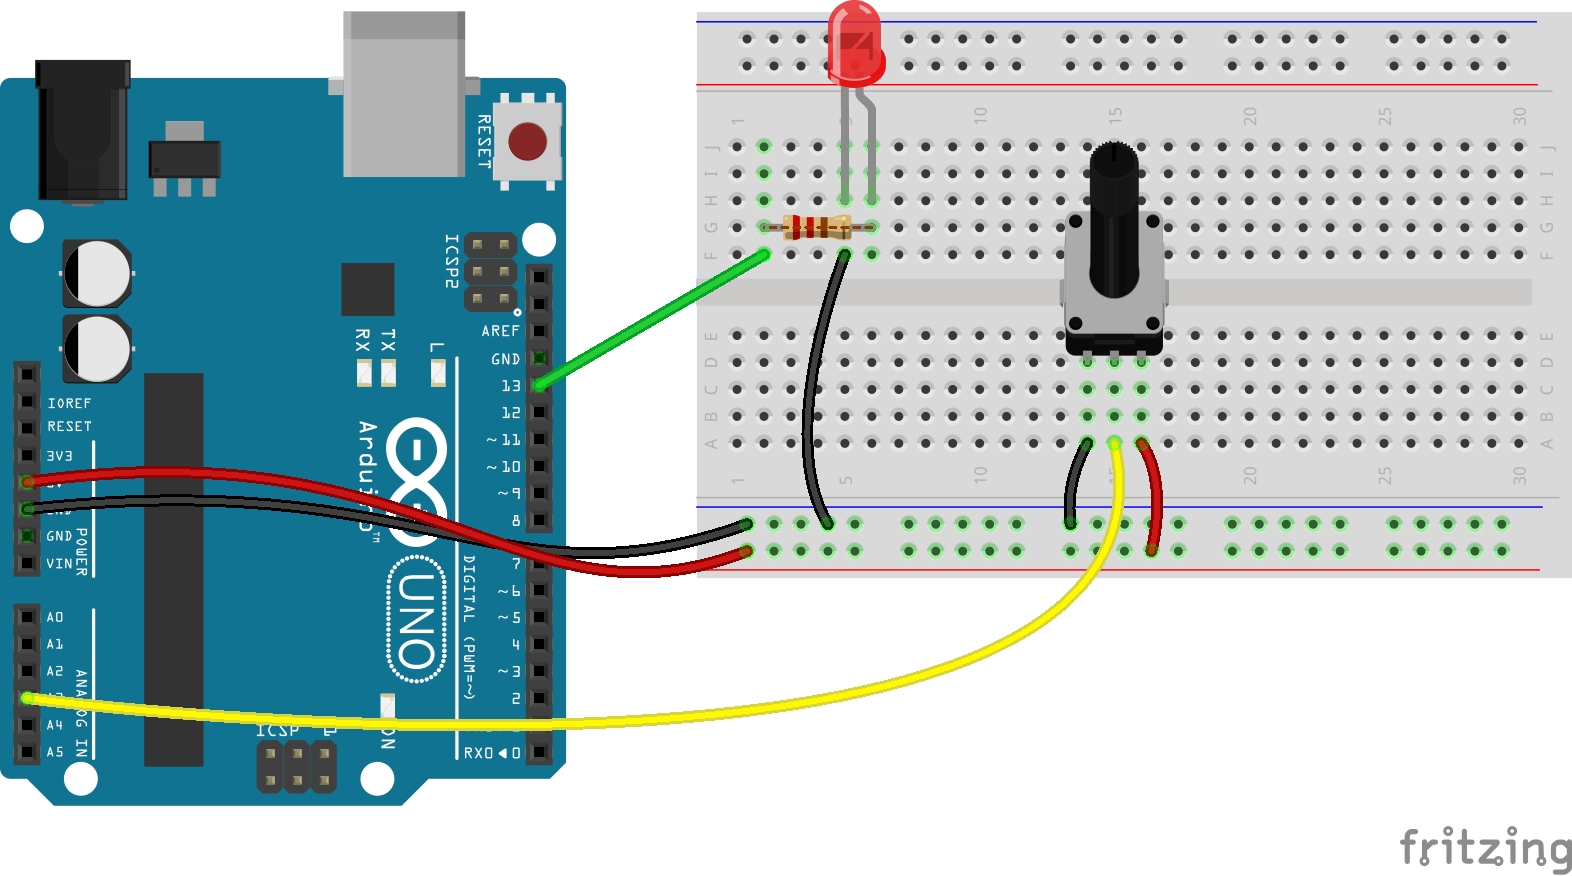
\includegraphics[width=0.6\linewidth]{graphics/fritzing_graphic.png}
  \captionof{figure}{An example Fritzing diagram.}
  \label{fig:fritz_graph}
\end{figure}

Fritzing\footnote{http://fritzing.org/home/} is open-source software that (among other uses) enables the user to create circuit diagrams and export a netlist\footnote{An XML file encapsulating all the parts and connections in the circuit}. Figures \ref{fig:fritz_graph} and \ref{fig:fritz_net} show a Fritzing diagram and part of a netlist for that diagram. The goal of the Fritzing netlist analysis component is to make it simpler to handle cases where the source and target platform have different pin configurations for a functionally equivalent circuit. For example, an LED may be attached to pin 12 on the source board and pin 6 on the target. Manually changing the references to this pin number can be error prone. Given a Fritzing netlist and a config file (containing additional information about Fritzing parts) this component calculates which pin of the board each part is connected to. This information is passed to the Code Generation EGL transform and used to generate pin variables in the output file.

\begin{figure}[h!]
  \centering
  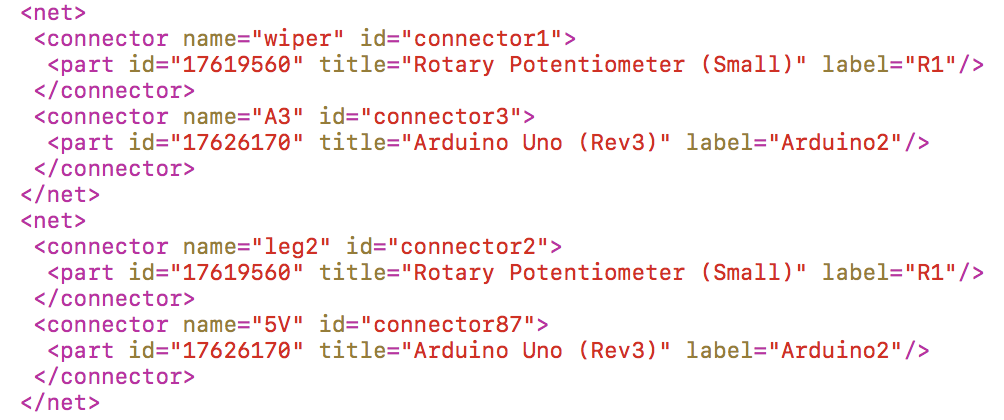
\includegraphics[width=0.8\linewidth]{graphics/fritzing_netlist.png}
  \captionof{figure}{Part of the netlist generated for Figure \ref{fig:fritz_graph}.}
  \label{fig:fritz_net}
\end{figure}

The goal of the Arduino libraries analysis component is to aid in mapping between source and target platform libraries. This is acheived by suggesting to the user suitable target platform libraries for the parts in the Fritzing netlist. Analysis is performed based on these parts and the Arduino header files to propose suitable libraries. Additionally, chosen libraries are recorded in the config. file and this is used to inform the suggestions when the system is run subsequently. The libraries chosen by the user are passed to the Code Generation EGL transform and used to add suitable include statements to the output file.

Finally, the goal of the Parallax source analysis component is to take the code for the source platform and modify it to make it suitable for the target platform and indicate any areas of the code that need manual modification. Source-platform-dependent constructs are identified during the analysis and this information is passed to the Code Generation EGL transform. Code that does not need modification is passed as is. For example, the method signatures of source platform library function calls are identified in the analysis. These signatures are then used to generate empty method stubs in the output file with TODO directives indicating these need to be manually replaced.

\subsection{Design Rationale}
Based on the requirements and stakeholders outlined in Chapter \ref{reqs}, reusability and modifiability were identified as the key quality attributes for the system. Based on the potential usage of Software Obsolescence Researchers, it is important that the system exhibits reusability so that successful components of the system are able to be used easily within other projects. As such, the system was designed to have loose coupling between components, in particular the three main components shown in Figure \ref{fig:high_level_overview}. This diagram clearly shows each of these elements works independently of the others and so could easily be reused. 

It is also crucial that the system displays a high degree of modifiability to support requirement S-2: ``\textit{Users can easily adapt the system to support migration of software between different microprocessors.}''. This is again supported by loose coupling between components. Another decision to support modifiability was to use a configuration file as input to the components analysing the Fritzing netlist and Arduino libraries. This file contains information that could have been hardcoded into each component. However, using a configuration file allows this to be easily replaced for supporting migration between different platforms.

\section{Fritzing Netlist Analysis} \label{fritz_design}
\begin{figure}[h!]
  \centering
  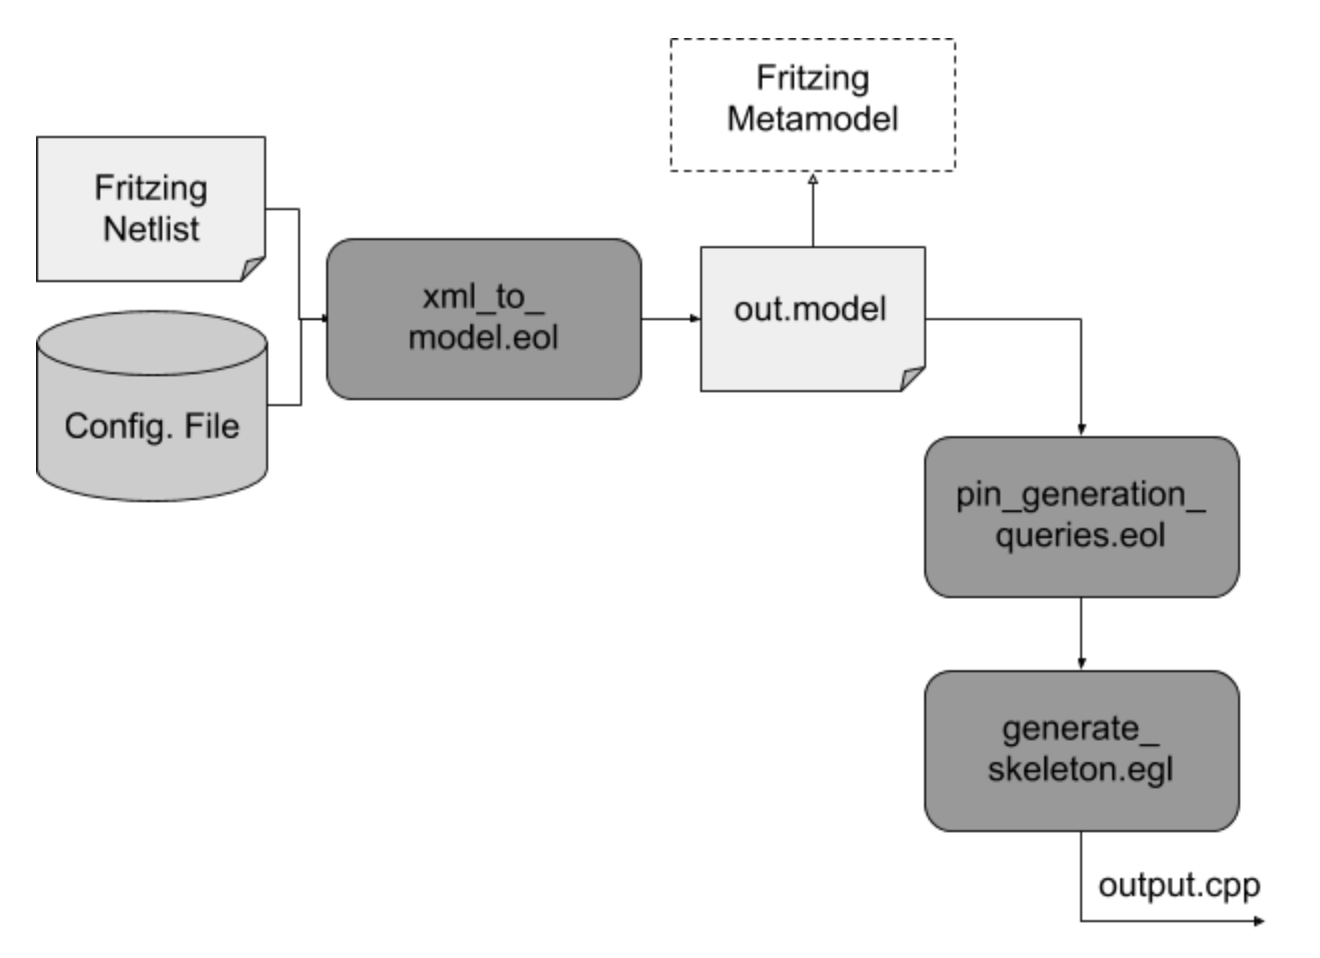
\includegraphics[width=0.8\linewidth]{graphics/fritzing_analysis.png}
  \caption{A more detailed view of the Fritzing netlist analysis component of the system.}
  \label{fig:fritzing_analysis}
\end{figure}

\subsection{Design}
The Fritzing netlist analysis component first consists of an XML to model transformation to extract the key information from the netlist. EOL queries are applied to this model to extract the connections from the parts to the target board. The Code Generation transform uses these queries in generating the pin variables for the output.

Although the netlist could be queried directly, the resulting model contains the information in a format making the queries easier to write as well as combining information from the config. file. This adds extra processing time but makes the code easier to understand which is more important given the requirements for the system.

Similarly, the output model from the transform could have been queried directly from the Code Generation EGL transform rather than having a separate EOL file to perform the queries. However, separating out the queries makes the logic in the EGL transform simpler as well as helping decouple the code generation from the implementation of the model/query logic. This improves the modifiability and reusability of this component.

\subsection{Implementation}

\begin{figure}[h!]
  \centering
  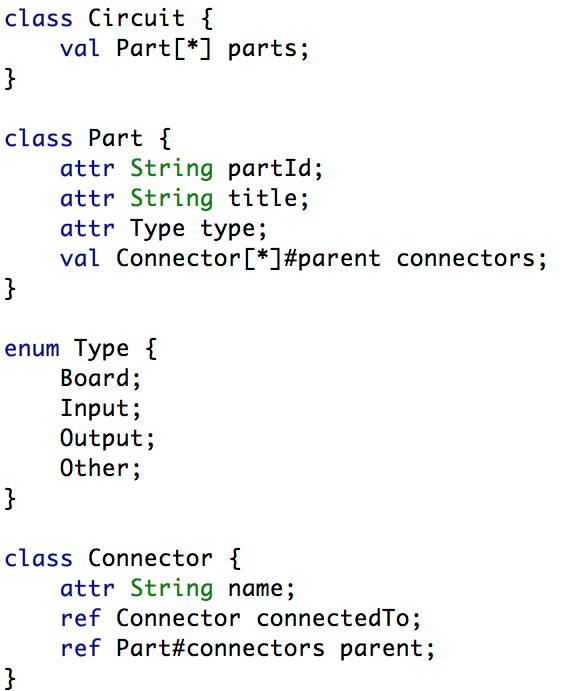
\includegraphics[width=0.4\linewidth]{graphics/fritz_metamodel.png}
  \caption{The EMF representation of the Fritzing metamodel.}
  \label{fig:fritz_metamodel}
\end{figure}

\subsubsection{Model Transform and Metamodel Design}
Figure \ref{fig:fritz_metamodel} shows the format for the Fritzing metamodel shown in Figure \ref{fig:fritzing_analysis}. The metamodel captures the essential information required to resolve the connections from parts to the Arduino board. Models conforming to this metamodel represent the circuit as a graph where nodes are parts and edges represent connections between the connectors of these parts. A graphical example of a model for the circuit in Figure \ref{fig:fritz_graph} is shown in Figure \ref{fig:fritz_model}.

\begin{figure}[h!]
  \centering
  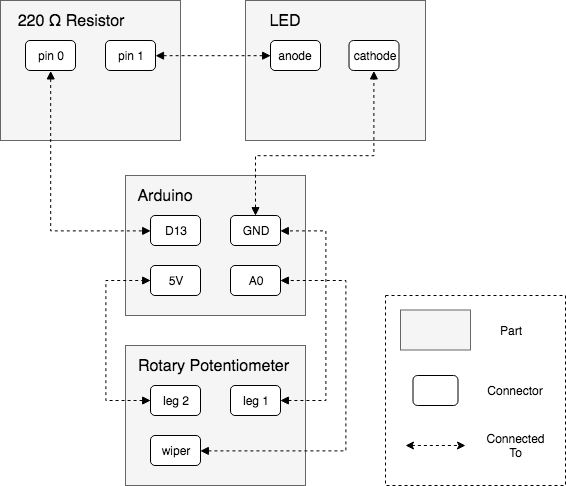
\includegraphics[width=0.6\linewidth]{graphics/fritz_model.png}
  \caption{A graphical representation of the model conforming to the metamodel shown in Figure \ref{fig:fritz_metamodel} for the circuit shown in Figure \ref{fig:fritz_graph}.}
  \label{fig:fritz_model}
\end{figure}

Most of the information for instantiating these models is extracted directly from the netlist. However, additional information about the type of parts is required. For example, when creating the pin variables in the output, we only want to generate values for devices read/written by the Arduino such as LEDs or potentiometers. Other parts, such as resistors, should not have pin variables generated. The config file (an example can be seen in Figure \ref{fig:config}) contains mappings between Fritzing part names and the type of the part. The part type is used to indicate whether or not variables should be generated for this component in the output file. This type information is stored as an attribute of the Part class in the model and is taken into account by the queries used to generate pin variables.

\begin{figure}[h!]
  \centering
  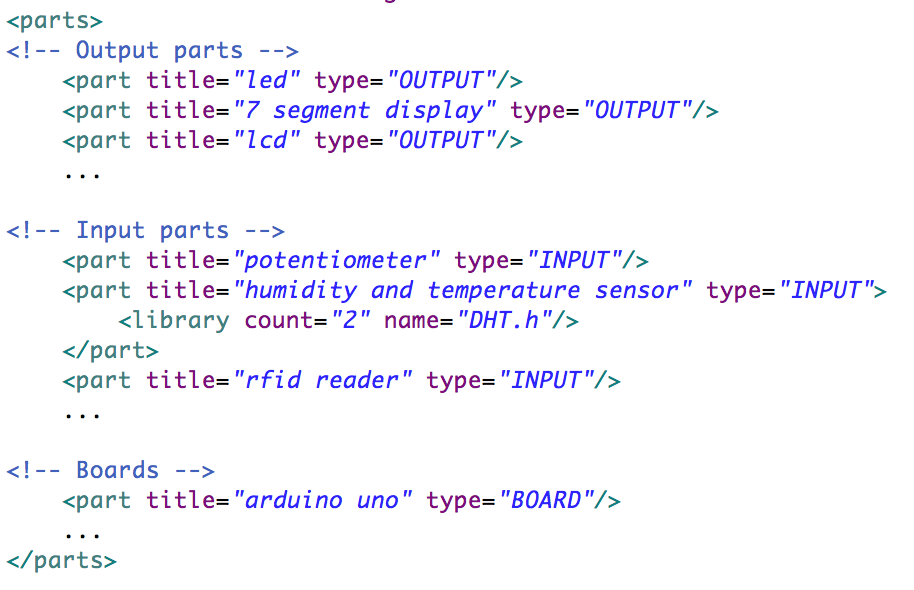
\includegraphics[width=0.6\linewidth]{graphics/config_file.png}
  \caption{Structure of the config file.}
  \label{fig:config}
\end{figure}

\subsubsection{Pin Generation Queries}
To find out which pins of the board parts in the circuit are connected to, a modified breadth-first search is performed on the Fritzing model. For each of the I/O connectors on the board, the connections in the model are followed until an input/output part is found. For example, resolving the connection to digital pin 13 (D13) in Figure \ref{fig:fritz_model} follows the connection to pin 0 of the 220$\Omega$ resistor, sees that this not an input/output part so follows the outgoing connections from this component (i.e. pin 1) to the anode of the LED. As this is a part tagged as an output type, a variable is then generated associating the LED with pin 13 on the Arduino board. The pseudocode below demonstrates the algorithm used for resolving the connections from the board to the input/output parts.

\begin{algorithm}
\begin{algorithmic}[1]
\Procedure{resolveBoardConnections}{}
\For{$connector$ in $board.connectors$} 
\State $connectedSensor \leftarrow bfsResolveConnections(connector)$
\State $connections.put(connector, connectedSensor)$
\EndFor
\Return $connections$
\\
\EndProcedure
\Procedure{bfsResolveConnections}{}

\EndProcedure
\end{algorithmic}
\end{algorithm}
% TODO: test assumption about only one component to each pin/
% TODO: include pseudocode for resolving pin connections

\section{Arduino Library Analysis}
\begin{figure}[h!]
  \centering
  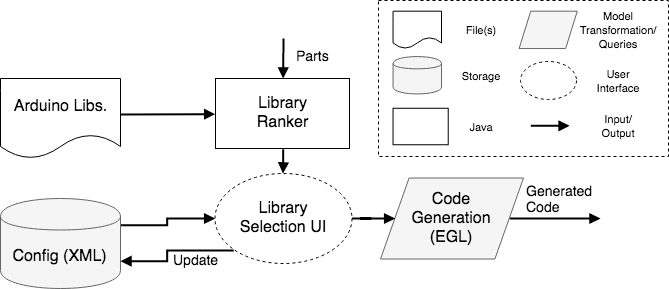
\includegraphics[width=0.8\linewidth]{graphics/arduino_library_analysis.png}
  \caption{A more detailed view of the Arduino library analysis component of the system.}
  \label{fig:arduino_analysis}
\end{figure}

\subsection{Design}
The Arduino Library Analysis component is used to suggest target platform libraries for each part in the Fritzing netlist. There are two methods used for library suggestion:
\begin{description}
\item[Library Ranker:] This treats library suggestion as an information retrieval task based on the part name. In other words, the Arduino libraries' header files are ranked based on similarity to the part's name. This makes the assumption that the most suitable library for a part will make some reference or include similar terms to the part's name. 
\item[Config:] The config. file stores information about the previously used libraries for a given part. For example, Figure \ref{fig:config} shows that the library "DHT.h" has been chosen twice for the humidity and temperature sensor. Whenever a library is chosen for a given part, the config file is updated with this choice.
\end{description}

The Library Selection UI combines the library suggestions and displays them to the user. Once the choices have been made, it also coordinates the update of the config file and passes on the library choices to the Code Generation EGL transform. As the only information passed to the Code Generation transform is a list of libraries, there is no separate EOL file used in this component unlike in the Fritzing netlist analysis component (e.g. the Pin Gen. Queries in Figure \ref{fig:fritzing_analysis}).

As these library suggestion sub-components are logically independent, they have been separated to improve modifiability and reusability. Furthermore, the use of the config handler between the library selection UI and the config file abstracts away from the format of this file. This makes it easier to modify this subcomponent. For example, changing the format of the config file will not require a change in the library selection UI.

\subsection{Implementation}
% TODO: add diagram of user library selection
\subsubsection{Library Ranker}
%TODO
\subsubsection{Config}
%TODO

\section{Parallax Project Analysis} \label{parallax_design}
\begin{figure}[h!]
  \centering
  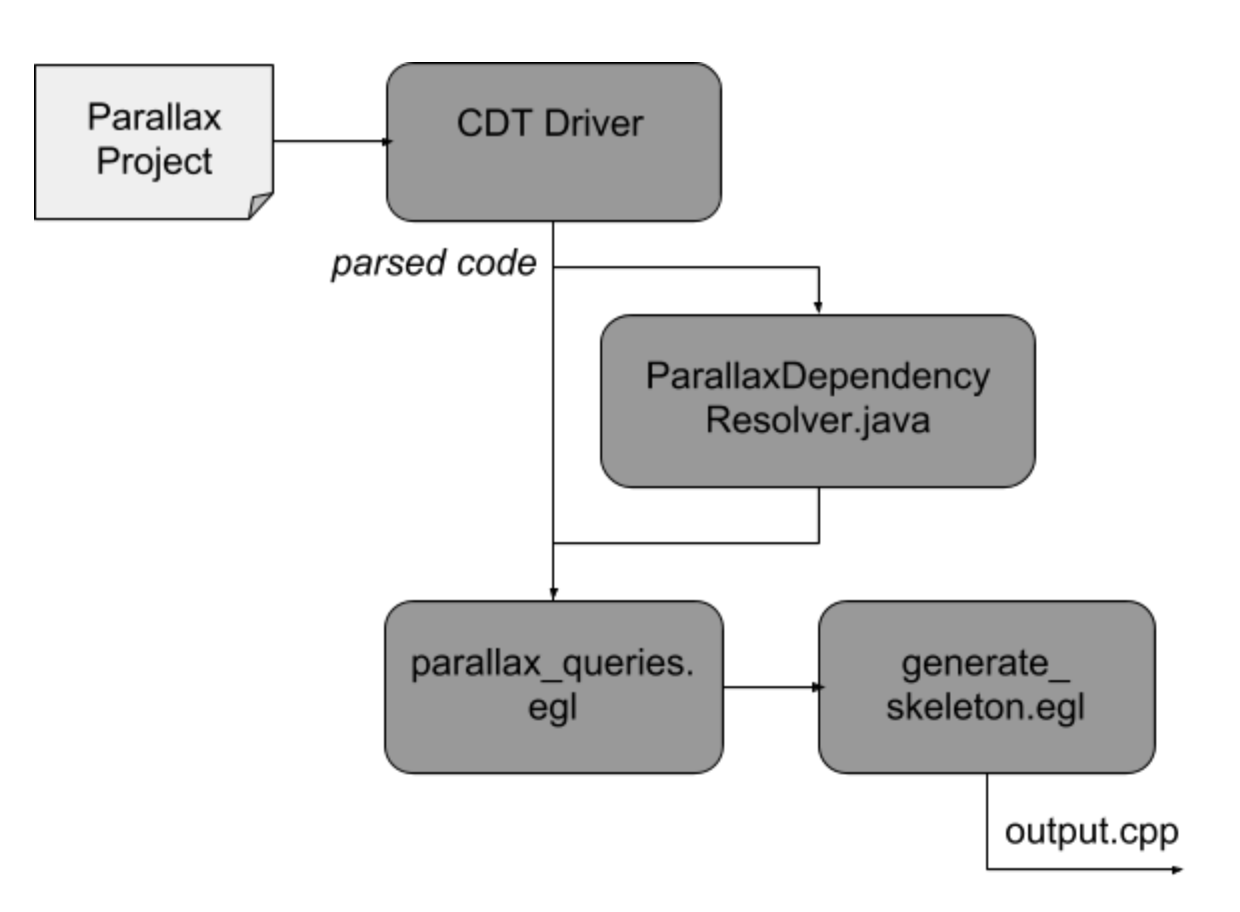
\includegraphics[width=0.8\linewidth]{graphics/parallax_project_analysis.png}
  \caption{A more detailed view of the Parallax project analysis component of the system.}
  \label{fig:parallax_analysis}
\end{figure}

\subsection{Design}
// TODO
\subsection{Implementation}
// TODO

\section{Limitations}
%TODO: limitations on LibraryRanker e.g. fritzing names are not always intelligible/no guarantee against clashes; intended to be a heuristic not a solution


\chapter{Evaluation}
%TODO

\chapter{Conclusion}
%TODO
%TODO discuss effort of testing

\printbibliography
\end{document}